Go to \url{https://sagecell.sagemath.org/}.

You can enter basic Sage commands into the textbox on the page and
click ``Evaluate'' to get the output.  To get started let's use sage like a fancy calculator.  The operands for sum, difference, multiplication, and division are \verb% +, -, *, / %.

Try the following operations:

\begin{enumerate}

	\item Try the following operations:
	\begin{enumerate}
		\item \verb% 1 + 2 + 3 %
		\item \verb% 42 - 23 %
		\item \verb% 1331 * 11 %
		\item \verb% 144 / 9 %
    \end{enumerate}

    \item That's pretty standard stuff, you could more easily do those on your phone\dots  But, can your phone calculate 200 digits of $\pi$ in the blink of an eye?  Try this:

\begin{codeblock}
\begin{verbatim}
n(pi, digits=200)
\end{verbatim}
\end{codeblock}

    \item You may have noticed that the previous question's answers were all whole numbers, but this last one was a decimal.  We've been holding out on you a bit -- sage does {\em exact} computations.  Unless you ask it for a numerical approximation (which is what the 
    {\tt n( )} function was all about) it will give answers that are 100\% precise -- but sometimes that doesn't seem very helpful!  

    \noindent Try evaluating these:
    \begin{enumerate}
		\item \verb% pi %
		\item \verb% sqrt(2) %
		\item \verb% 7/3 %
    \end{enumerate}

    \item Sage and its brethren are Symbolic Computer Algebra Systems.  The reason it just parrots back the question to you has to do with the ``Symbolic'' part of that.  For example, the \verb+sqrt(2)+ thing above is regarded by Sage as a symbolic entity.  It is a full and precise representation of the number we write as $\sqrt{2}$.  It isn't some lame 4 or 10 or 100 digit {\em approximation} of $\sqrt{2}$. It is the real deal.  Let's see what happens when we raise \verb+sqrt(2)+ to various powers (you can use either \verb+^+ or \verb+**+ for exponentiation in sage).

	\noindent Try evaluating these:
    \begin{enumerate}
		\item \verb% sqrt(2) ^ 2 %
		\item \verb% sqrt(2) ^ 4 %
		\item \verb% sqrt(2) ^ 7 %
    \end{enumerate}

    \noindent Was the answer to that last one suprising?  Or does it make sense in retrospect?

    \item Much of the power of Computer Algebra comes from the same feature that makes regular Algebra useful -- variables.

    \noindent There are two kinds that we need to distinguish: computer variables and mathematical variables.  Computer variables are pretty easy, you can just make up whatever name you want and then start using it.  For example:

\begin{codeblock}
\begin{verbatim}
myvar = sqrt(2) ^ 7
n(myvar)
\end{verbatim}
\end{codeblock}

\noindent BTW, notice how the default version of the  {\tt n()} function only gives about 13 decimal places?  Try this too: \verb+ n(myvar, 100)+ (that's what 100 {\em bytes} of accuracy looks like -- if you want a specific number of decimal places, see the example involving $\pi$ up above.)

	\item Mathematical variables are handled a little differently.  First (other than $x$ which is there automatically) you have to declare them to the system.  The syntax looks like this: \verb+ y = var('y')+.  What's happening there is that we're telling the system that {\tt y} is a variable, but also that we want the system to print 'y' when referring to it.  I think you'll get the point if you figure out what happens when you evaluate \verb+ y = var('w') ; 6*y+.

	\item Let's try a little mathy something - with a couple of variables.  Remember how the equation of a line is usually written as $y = mx + b$?  Put the following into the sage cell:

\begin{codeblock}
\begin{verbatim}
y=var('y')
m = 2 ; b = 1
y=mx+b
\end{verbatim}
\end{codeblock}

The error message you get when evaluating this should look like:

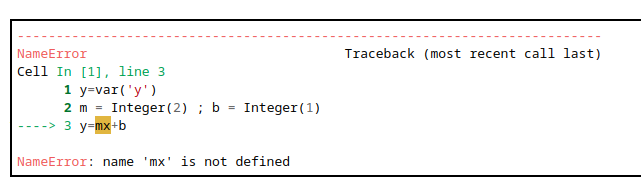
\includegraphics[scale=.5]{sage_cell-error.png}

To be fair, Sage usually puts out error messages that are on the cryptic side.  But not this time!  The message says ``NameError'' and it's even highlighted the thing that's wrong. \footnote{A takeaway from this is that you can't rely on implicit multiplication.  If you write \verb+7x+ the system is going to think you've created a new (computer) variable whose name is ``7x.''  What you really {\em meant} was \verb+7*x+ and that's what you have to actually type!} 

If you fix the error, something else a little unexpected happens. Nothing!  There's no output\dots

This is just because the last line is an assignment -- it has no return value.  A very common ``idiom'' you'll see when looking at other people's sage code looks like this:

\begin{codeblock}
\begin{verbatim}
y=var('y')
m = 2 ; b = 1
y=mx+b ; y
\end{verbatim}
\end{codeblock}

\noindent The semicolon is just a way to sneak multiple commands onto a single line.  The difference here (as opposed to the code above) is that the last command isn't the assignment to the variable \verb+y+, it's just \verb+y+ by itself - and that does have a return value, namely the contents of the variable \verb+y+.



	\item Calculate $2^0$, $2^0+2^1$, $2^0+2^1+2^2$, 
		and $2^0+2^1+2^2+2^3$. Continue adding the next
		largest power of $2$ until you notice a pattern in the
		result. What is the pattern?
	
\end{enumerate}

m=2; b=1;
y=mx+b



